\paragraph{QuizziPedia::Front-End::Views::HomeView}

\label{QuizziPedia::Front-End::View::HomeView}
\begin{figure} [ht]
	\centering
	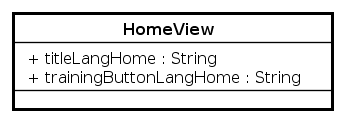
\includegraphics[scale=0.80]{UML/Classi/Front-End/QuizziPedia_Front-end_Views_HomeView.png}
	\caption{QuizziPedia::Front-End::Views::HomeView}
\end{figure} \FloatBarrier
\begin{itemize}
	\item \textbf{Descrizione}: \textit{view\ped{G}} contenente la direttiva per barra di ricerca degli utenti e questionari e il bottone che porterà l'utente nella modalità allenamento;
	\item \textbf{Utilizzo}: viene utilizzata come \textit{view\ped{G}} iniziale dell'applicazione;
	\item \textbf{Relazioni con altre classi}:
	\begin{itemize}
		\item \textbf{IN \texttt{HomeModelView}}: classe di tipo \textit{modelview\ped{G}} la cui istanziazione è contenuta all'interno della variabile di ambiente \$scope di \textit{Angular\ped{G}}. All'interno di essa sono presenti le variabili e i metodi necessari per il \textit{Two-Way Data-Binding\ped{G}} tra la \textit{view\ped{G}} \texttt{HomeView} e il \textit{controller\ped{G}} \texttt{HomeController};
		\item \textbf{IN \texttt{SearchDirective}}: directive che permette di effettuare la ricerca di utenti e questionari;
		\item \textbf{IN \texttt{LangModel}}: rappresenta il modello delle informazioni per la giusta traduzione dell'applicazione.
	\end{itemize}
	\item \textbf{Attributi}:
	\begin{itemize}
		\item \texttt{+ titleLangHome: String} \\ Attributo che viene utilizzato per visualizzare la giusta traduzione del titolo della pagina, in italiano o in inglese;
		\item \texttt{+ trainingButtonLangHome: String} \\ Attributo che viene utilizzato per visualizzare la giusta traduzione della \textit{label\ped{G}} per il bottone di link alla modalità allenamento, in italiano o in inglese.
	\end{itemize}
\end{itemize}
	